%Documentação do Trabalho Prático 0 de AEDSIII
%Édipo Fernandes Vieira de Oliveira - 2011054324
\documentclass[12pt, a4paper]{article}
\usepackage[utf8]{inputenc}
\usepackage[brazil]{babel} %idioma
\usepackage{ae} %caracteres especiais
\usepackage{amsmath, amsfonts, amssymb}
\usepackage{enumerate}
\usepackage[tmargin=2cm, bmargin=2cm, lmargin=2cm, rmargin=2cm]{geometry}
\usepackage{graphicx}
\usepackage[lined,algonl,ruled]{algorithm2e} %Para acrescentar algorithm
\begin{document}

 %capa

 \title{Trabalho Prático 2 \\ Jogo de Baralho - Burro \\}
 \author{Édipo Fernandes Vieira de Oliveira - 2011054324\\ Diego Henrique de Castro Aniceto - 2011054286\\Departamento de Ciência da Computação -- Universidade Federal de Minas Gerais\\}
  \maketitle

 %\newpage
 %sumario
  %use o section

\textbf{\textit \\Resumo: }
\textit{\\ Este relatório descreve a implementação do Jogo de baralho Burro. Para que fosse possivel essa implemetação foi utilizado a linguagem de programação Java além de teorias de Orientação a Objeto, dentre elas Modularização, Encapsulamento, Herança, Polimorfismo, entre outras.\\
  O resultado obtido foi satisfatório, tanto em relação a solução do problema, quanto aos conceitos envolvidos.}
\section*{1. Introdução}

  Este trabalho tem como objetivo, observar na prática os principais conceitos da Programação Orientada ao Objetoo. Para que estes fossem exercitados foi proposto a implementação de um jogo de baralho. O jogo escolhido é chamado \textbf{Burro}, um jogo simples jogado por no minimo duas pessoas, sem limite máximo de jogadores.
  \\\\
  O jogo foi modelado utilizando como base as entidades principais do jogo, \textit{Jogador} e \textit{Baralho}, e a partir destas foram geradas as classes utilizadas para o desenvolvimento do jogo e que também serão descritas nas próximas sessões.
  \\\\
  Para que a implementação deste trabalho fosse possível, foram utilizados conceitos de Orientação a Objeto, como herança, polimorfismo, restrição de acesso, entre outros, pois dessa forma o algoritmo cobre os requisitos básicos solicitados e também facilita a compreensão do trabalho.
  \\\\
  O trabalho está composto das seguintes seções:\\\\
  \begin{itemize}
    \item A seção 2 discute detalhes de implementação e da modelagem do problema.
    \item A seção 3 traz os testes realizados para verificar a solução do trabalho, bem como a saída gerada
    \item A seção 4 apresenta uma breve conclusão sobre o trabalho.
    \item E por fim a seção 5 traz as referências bibliográficas.
  \end{itemize}

%% Implementação %%
\section*{2. Implementação}
  \subsection*{2.1. Modelagem do Jogo}
  O jogo foi modelado em torno de duas classes principais, \textit{Jogador} e \textit{Baralho}.
  \\\\
  A classe \textit{Jogador} é abstrata, logo contem métodos abstratos e concretos, ela também é a classe base de outras duas, \textit{JogadorHumano} e \textit{JogadorBot} que extendem da super classe. A classe \textit{JogadorHumano} como o proprio nome diz, modela um jogador humano e de acordo com o conceito de herança, ela "É-UM" \textit{Jogador}, assim ela só pode ser um jogador  e a classe \textit{JogadorBot} modela um jogador controlado pelo computador e segue o mesmo conceito da classe anterior, porém essa classe não foi complemtamente implementada.\\\\
  A classe \textit{Baralho} é uma classe concreta que é composta por \textit{Cartas}, estas por sua vez são compostas de \textit{Naipe} e \textit{Valor}, essas duas ultimas, são enumerações, uma forma encontrada para facilitar o desenvolvimento e deixa-lo mais simplificado.
  \\\\
  Essa modelagem pode ser visualizada de forma simples no Diagrama de Classes a seguir:
%% Inserir a baixo o Diagrama de Classes  =================================================================================

  \begin{figure}[!htb]
   \centering
   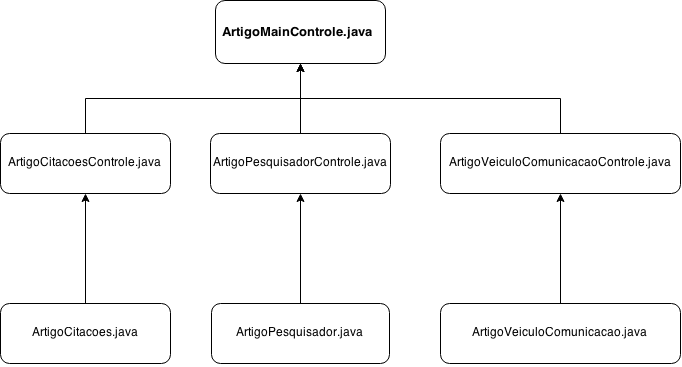
\includegraphics[scale=0.5]{Artigo}
   \caption{Diagrama de Classes}
   \label{Rotulo}
  \end{figure}
%% ========================================================================================================================


  São necessários no mínimo duas pessoas para jogar, porém não contém um numero máximo de jogadores. O jogo se inicia com as pessoas recebendo quatro cartas cada, uma destas deverá jogar uma carta na mesa, as demais deverão jogar uma carta do mesmo naipe daquela que está na mesa, caso não tenham o naipe solicitado em mãos a pessoa deverá comprar cartas no monte de cartas ate que encontre o naipe necessário, quem jogar a maior carta será  vencedor da jogada, e deverá iniciar a próxima rodada. O vencedor do será aquele que jogar todas as suas cartas da mão na mesa. O perdedor será aquele que ficar com cartas na mão por ultimo. o numero de cartas que estiver na mão dele serão os 'anos de burrice' da pessoa.

 %% Inserir a baixo o Diagrama de Atividades ==============================================================================

  \begin{figure}[!htb]
   \centering
   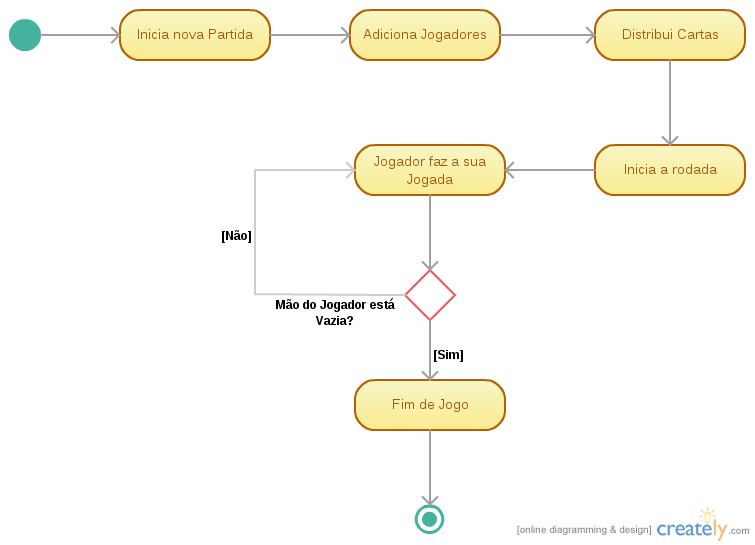
\includegraphics[scale=0.5]{DiagramaAtividadesBurro}
   \caption{Diagrama de Classes}
   \label{Rotulo}
  \end{figure}
%% ========================================================================================================================

   \subsection*{2.2. Conceitos OO}
    Foram utilizados para o desenvolvimento do produto final varios conceitos de orientação objeto.
    Dentre eles, foi utilizado o conceito de \textbf{Herança} para especificar a hierarquia de classes envolvendo as classes
    \textit{Jogador}, \textit{JogadorHumano} e \textit{JogadorBot}, onde a classe jogador contem dados mais gerais que ambos podem

   \subsection*{2.3. Calculos e Execução}

%% Testes %%
\section*{3. Testes}

%% Conclusão %%
\section*{4. Conclusão}


%% Referencias %%
\section*{5. Referências bibliográficas}
\end{document}
